
\newpage
\section{Design}
`Mobile phone adoption presents us with highly available, contextually aware and interactive platforms' \cite{article_mhealth}. Research into designing systems for mobile behaviour change technology, presents us with some implementation design requirements. Implementing a chatbot using these design considerations produces a solid ground for building this system.

\subsection*{Design Process}
Current mobile systems use apps to interact with users, but a recent study (2013) showed apps fall into a low behavioural theory adherence scale \cite{article_mhealth}. Research into how to build systems that are theory-based, suggest four main stages for designing mobile health solutions. Conceptualisation, Formative Research and Pretesting, Pilot trails and Evaluation trials \cite{article_mhealth}. The first two stages use the Behaviour Change Wheel \cite{article_behaviour_change_wheel} (a framework for planning health behaviour interventions), to understand the behaviour, better define the characteristics and form the mobile concept into a prototype. The pilot trials tests the prototype before it moves to a finalised app with the commitment of a full trail. The final stage tests the finalised app with a wider range of participants. This project will use these four stages as design steps to build the prototype.

\subsection*{Gamification Elements}
- Gamification elements \cite{article_free_to_play_making_money_from_games_you_give_away}
- Designing outstanding feedback loops \cite{website_how_to_design_feedback_loops}


\subsection{Implementing Rewards}
- Vision
  - Send notification
  - Show nice visuals

- Audio
  - Send notification
  - Play uplifting music

- Tactic
  - A.P.I. sets wearable alarm
  - Wearable (fitbit) issues and tracks alarm times

\subsubsection*{Methods of implementation}
- 3 Types:
  1. specific apps
    - Bad cuz takes a long time
  2. Web Apps
    - Still another app
  3. Chatbot
    - Good useful
- Android/iOS/chatbot specific notifications from web app
- Save to home screen

\subsubsection*{Technology}
Talk about different chatbot tech available, e.g. amazon lex, and why im choosing fb messenger
\url{https://aws.amazon.com/lex/}

Web app could be chosen because its easiest and achievable, however the ease of use with a chatbot, integrated into fb messenger means everyone can use it on multiple devices. The addition, means that people get used to the UI.

\subsection{Components}
  % [app] -------> (Database) -----> at certain time ---> Send notification to trigger type of reward
  % [ big button that says track]
  % taskname textbox

Flow diagram style
\tikzstyle{startstop} = [rectangle, rounded corners, minimum width=3cm, minimum height=1cm,text centered, draw=black, fill=red!30]
\tikzstyle{io} = [trapezium, trapezium left angle=70, trapezium right angle=110, minimum width=3cm, minimum height=1cm, text centered, draw=black, fill=blue!30]
\tikzstyle{process} = [rectangle, minimum width=3cm, minimum height=1cm, text centered, draw=black, fill=orange!30]
\tikzstyle{decision} = [diamond, minimum width=3cm, minimum height=1cm, text centered, draw=black, fill=green!30]
\tikzstyle{arrow} = [thick,->,>=stealth]

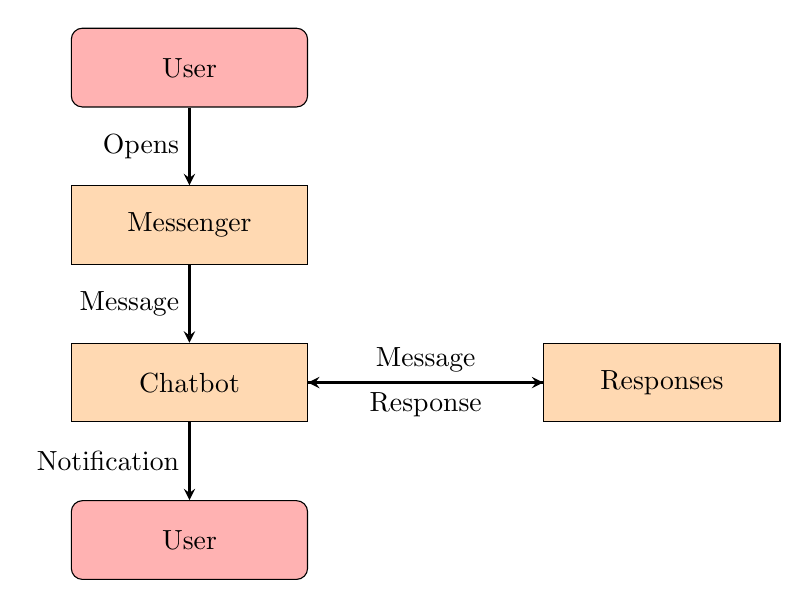
\begin{tikzpicture}[node distance=2cm]
  \node (user) [startstop] {User};
  \node (fbmsgr) [process, below of=user] {Messenger};
  \node (chatbot) [process, below of=fbmsgr] {Chatbot};
  \node (responses) [process, right of=chatbot, xshift=4cm] {Responses};
  \node (userend) [startstop, below of=chatbot] {User};

  \draw [arrow] (user) -- node[anchor=east] {Opens} (fbmsgr);
  \draw [arrow] (fbmsgr) -- node[anchor=east] {Message} (chatbot);
  \draw [arrow] (chatbot) -- node[anchor=south] {Message} (responses);
  \draw [arrow] (responses) -- node[anchor=north] {Response} (chatbot);
  \draw [arrow] (chatbot) -- node[anchor=east] {Notification} (userend);
\end{tikzpicture}

\subsection{Chatbots}

\subsubsection*{How 2 build and deliver these rewards to users}


\begin{figure}[ht] % ht
    \centering
    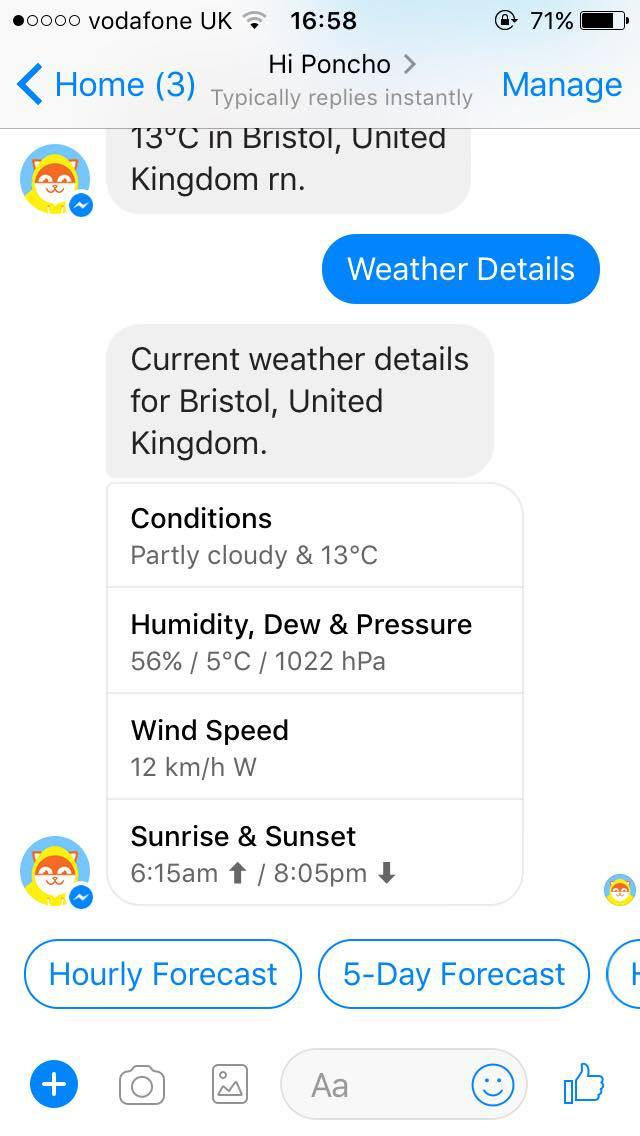
\includegraphics[width=3.2in]{../resources/poncho.jpg}
    \caption{Poncho: A Facebook Messenger Weather Chatbot}
    \label{fig:poncho}
\end{figure}

\subsubsection*{Current Chatbots}

  - Setup:
    - Setup the bot via a messaging platform, such as fb messenger
  - Trigger:
      - Either A, certain configured time of the day
      -        B: No trigger
      -        C: Around a specific time
  - Action:
    - Choose habit from list of habits
    - Perform
    - Use app to track the action
  - Reward:
    - You get one of these rewards, based on modalitiy selected
    - Vision
      - Through message, of an image or gif
      - Could be: App, or message, gif
    - Audatory
      - Through phone via bot, link to mp3/spotify/apple music
      - Could be: App
    - Tactic
      - Through wearable
      - Could be: App, bot triggers wearbale alarm

FB messenger


\subsubsection*{Training a chatbot}

\subsection{Design Requirements}

\subsection{Scope}

@TODO Scope and is the relevance of the reviewed work to the project is always made clear?


\subsection{User Flow}
  - Pre-Start
    - Choose daily habit type from list of X, e.g. 1 press up before breakfast
    - Enable notifications or fitbit if chosen
    - Time action / reward, variable rewards, e.g. then work out average time to send, or none
  - Start:
    - New day
    - @ trigger time, send reminder, if set, notification
    - Open notification, do habit, press tracked
    - Get reward type
